\subsection{Introduction}

\begin{frame}{Variational inference}
  \vspace{-10pt}
  \begin{itemize}[<+->]
    \item Name derived from calculus of variations which deals with maximising or minimising functionals.
    \begin{table}
      \begin{tabular}{l  l  l }
      Functions   &$p:\theta \mapsto \bbR$  &(standard calculus) \\ 
      Functionals &$\cH:p \mapsto \bbR$     &(variational calculus) \\ 
      \end{tabular}
    \end{table}
  \item Using standard calculus, we can solve
  \[
    \argmax_\theta p(\theta) =: \hat\theta
  \]
  e.g. $p$ is a likelihood function, and $\hat\theta$ is the ML estimate.
  \item Using variational calculus, we can solve
  \[
    \argmax_p \cH(p) =: \tilde p
  \]
  e.g. $\cH$ is the entropy $\cH = - \int p(x)\log p(x) \d x$, and $\tilde p$ is the entropy maximising distribution.
  \end{itemize}
  \vspace{5pt}
\end{frame}

\begin{frame}{Variational inference (cont.)}
  \blfootnote{\fullcite[Ch. 10]{Bishop2006}}
  \blfootnote{\fullcite[Ch. 21]{Murphy1991}}
  \vspace{-5pt}
  \begin{itemize}\setlength\itemsep{0.8em}
    \item Consider a statistical model where we have observations $(y_1, \dots, y_n)$ and also some latent variables $(z_1, \dots, z_n)$.
    \pause
    \item The $z_i$ could be random effects or some auxiliary latent variables.
    \item In a Bayesian setting, this could also include the parameters to be estimated.
    \pause
    \item \textbf{GOAL}: Find approximations for
    \begin{itemize}
      \item The posterior distribution $p(\bz|\by)$; and
      \item The marginal likelihood (or model evidence) $p(\by)$.
    \end{itemize}
    \item Variational inference is a deterministic approach, unlike MCMC.
  \end{itemize}
\end{frame}

\begin{frame}{Decomposition of the log marginal}  
  \vspace{-3pt}
  \begin{itemize}\setlength\itemsep{0.5em}
    \item Let $q(\bz)$ be some density function to approximate $p(\bz|\by)$. \pause Then the log-marginal density can be decomposed into
    \begin{align*}
      \log p(\by) &= \log p(\by,\bz) - \log p(\bz|\by) \\
      \onslide<3->{
      &= \int \left\{ \log \frac{p(\by,\bz)}{q(\bz)} - \log \frac{p(\bz|\by)}{q(\bz)} \right\} q(\bz) \d \bz \\    
      &=  \cL(q) +  \KL(q \Vert p) \\
      &\geq \cL(q) 
      }   
    \end{align*}
    \item<4-> $\cL$ is referred to as the ``lower-bound'', and it serves as a surrogate function to the marginal.
    \item<4-> Maximising $\cL(q)$ is equivalent to minimising $\KL(q \Vert p)$.
    \item<4-> Although $\KL(q \Vert p)$ is minimised at $q(\bz) \equiv p(\bz|\by)$ (c.f. EM algorithm), we are unable to work with $p(\bz|\by)$.
  \end{itemize}
\end{frame}

\begin{frame}{Comparison of approximations (density)}
  \vspace{-5pt}
  \only<1|handout:0>{
    \begin{center}
      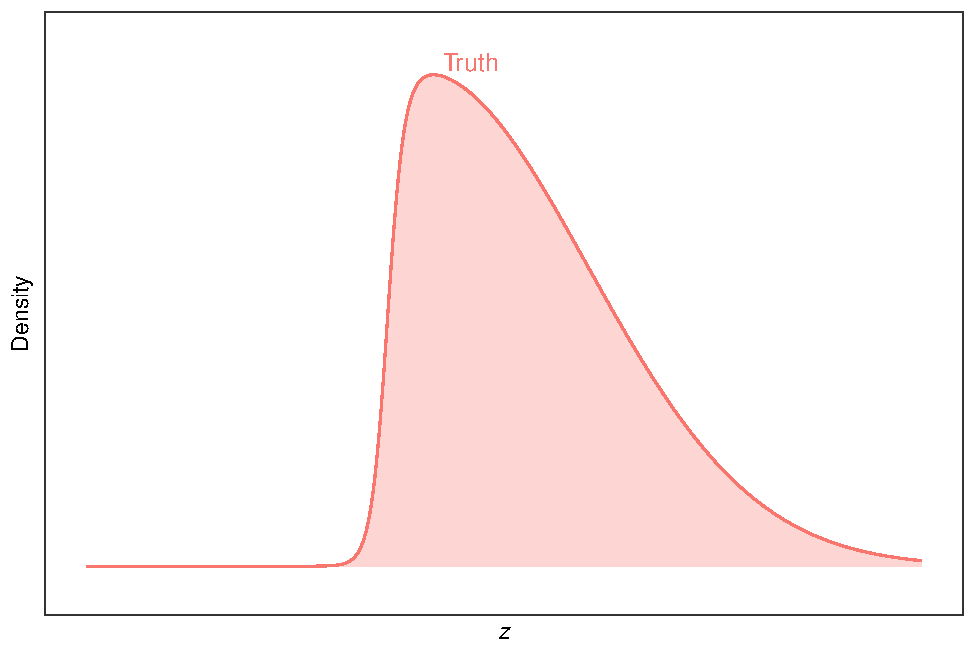
\includegraphics[scale=0.7]{figure/compare1}
    \end{center}
  }
%  \only<2|handout:0>{
%    \begin{center}
%      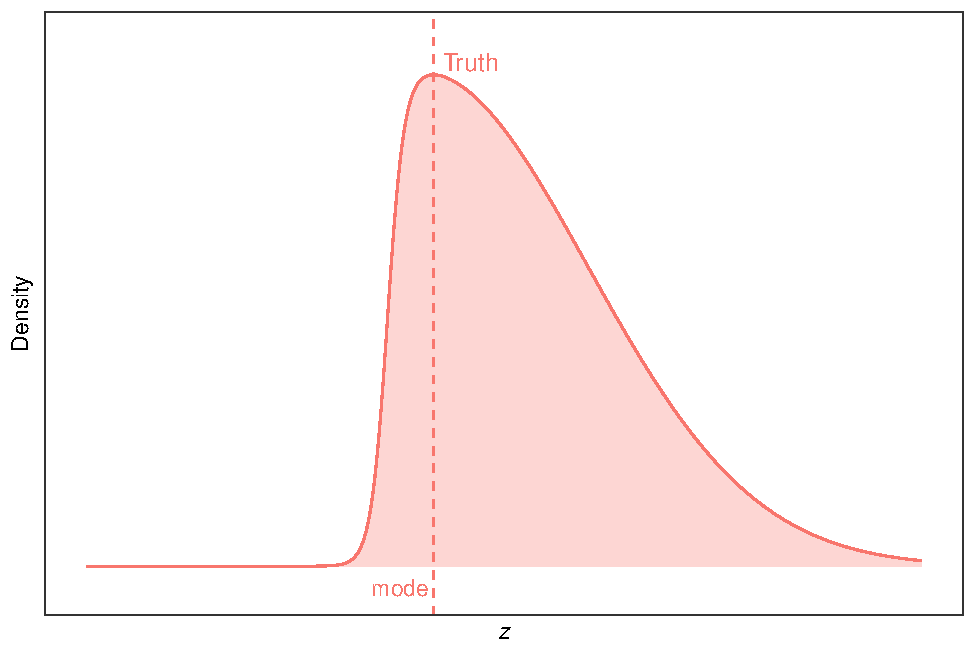
\includegraphics[scale=0.7]{figure/compare2}
%    \end{center}
%  }  
  \only<2|handout:0>{
    \begin{center}
      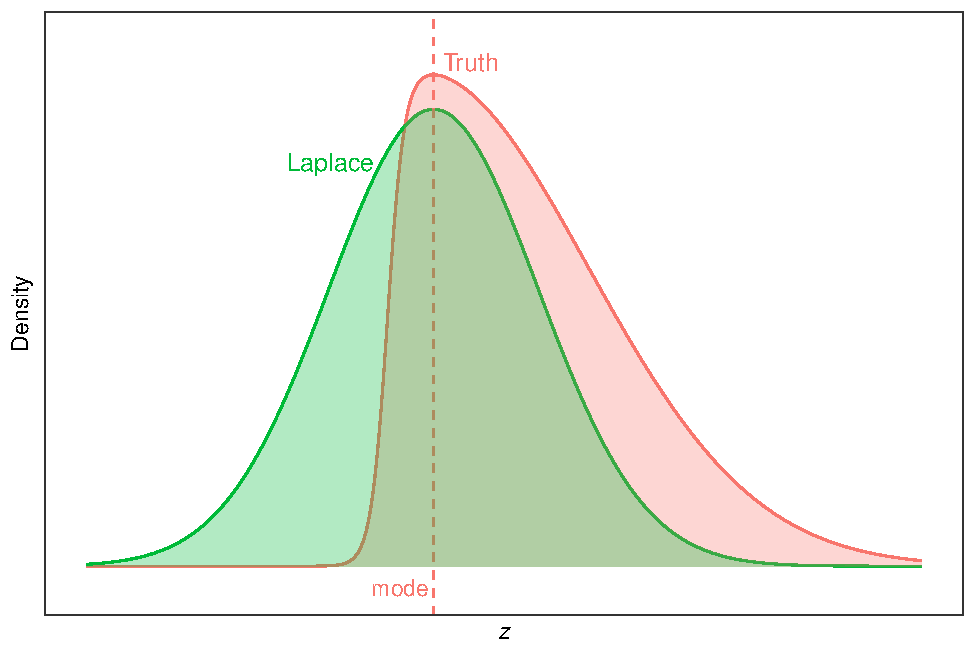
\includegraphics[scale=0.7]{figure/compare3}
    \end{center}
  } 
%  \only<4|handout:0>{
%    \begin{center}
%      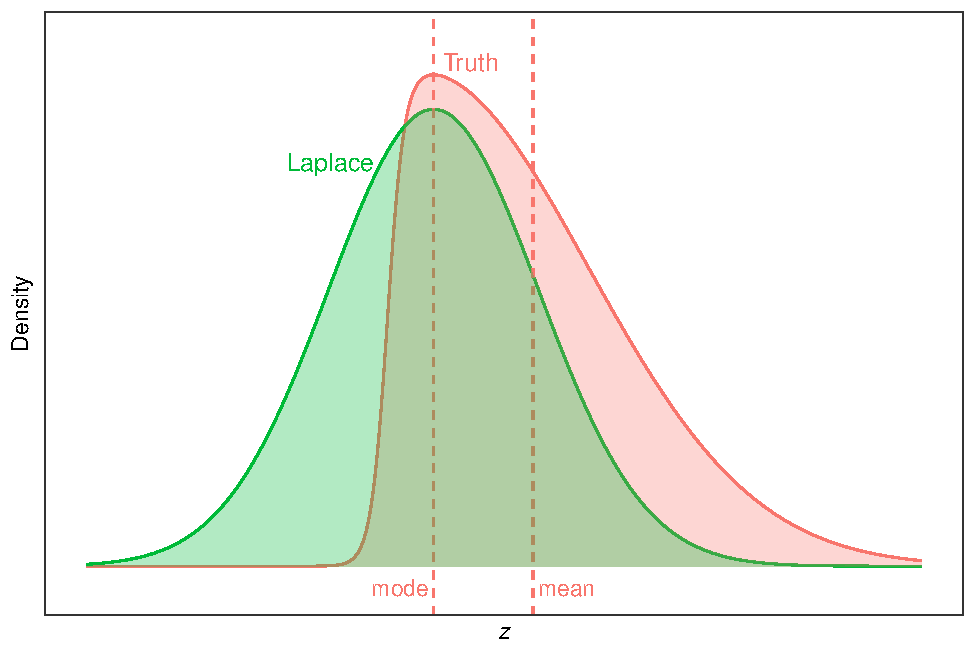
\includegraphics[scale=0.7]{figure/compare4}
%    \end{center}
%  } 
  \only<3|handout:1>{
    \begin{center}
      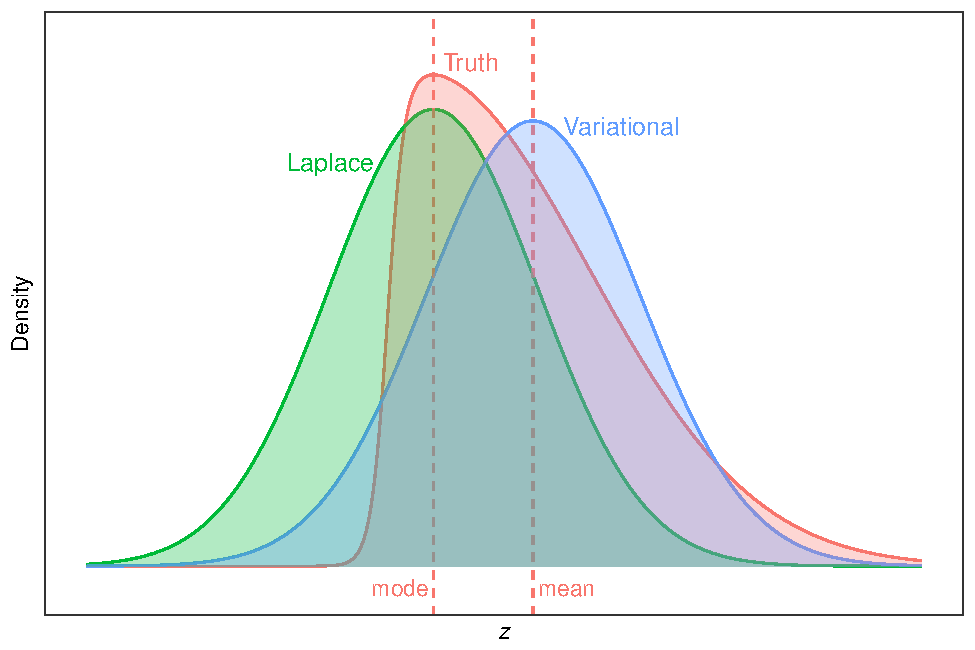
\includegraphics[scale=0.7]{figure/compare5}
    \end{center}
  } 
\end{frame}

\begin{frame}{Comparison of approximations (deviance)}
  \vspace{-5pt}
  \begin{center}
    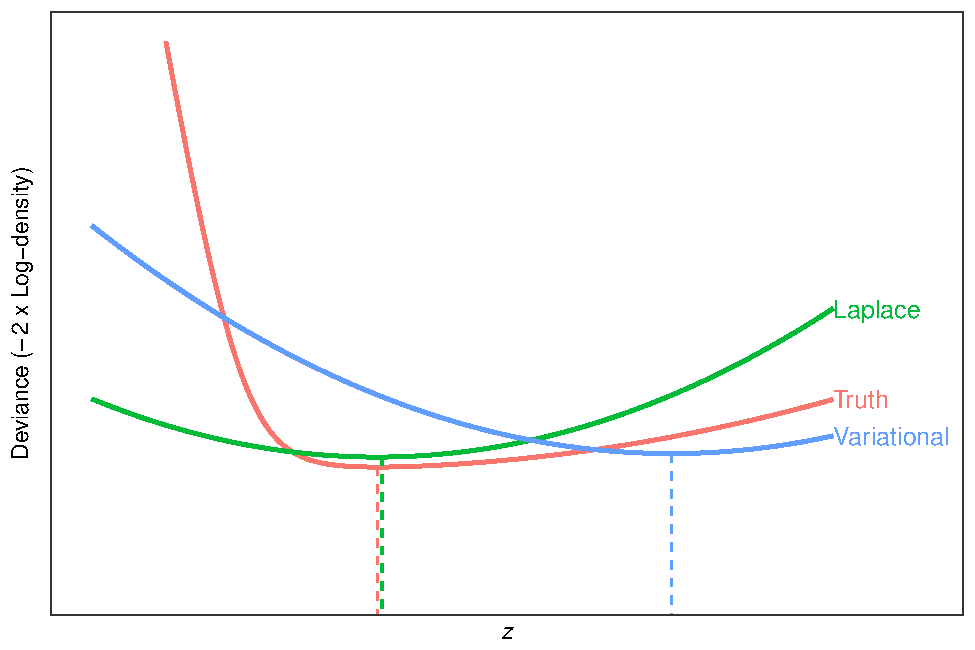
\includegraphics[scale=0.7]{figure/compare6}
  \end{center}
\end{frame}

\begin{frame}{Factorised distributions (Mean-field theory)}
  \blfootnote{\fullcite{Blei2016}}
  \vspace{-20pt}
  \begin{itemize}
    \item<1-> Maximising $\cL$ over all possible $q$ not feasible. Need some restrictions, but only to achieve tractability.
    \item<1-> Suppose we partition elements of $\bz$ into $m$ disjoint groups $\bz = (\bz^{(1)}, \dots, \bz^{(m)})$, and assume
    \[
      q(\bz) = \prod_{j=1}^m q_j(\bz^{(j)})
    \]
    \item<2-> Under this restriction, the solution to $\argmax_q \cL(q)$ is
    \begin{align}\label{eq:meanfieldsoln}
      \tilde q_j(\bz^{(j)}) \propto \exp\big(\E_{-j}[\log p(\by,\bz)]\big)
    \end{align}
    for $j \in \{1,\dots,m\}$.
    \item<3-> In practice, these unnormalised densities are of recognisable form (especially if conjugate priors are used).
    \vspace{4pt}
  \end{itemize}
\end{frame}

\begin{frame}{Coordinate ascent mean-field variational inference (CAVI)}
  \vspace{-5pt}
  \begin{itemize}\setlength\itemsep{0.4em}
    \item The optimal distributions are coupled with another, i.e. each $\tilde q_j(\bz^{(j)})$ depends on the optimal moments of $\bz^{(k)}$, $k \in \{1,\dots,m:k \neq j\}$.
    \item One way around this to employ an iterative procedure.
    \item Assess convergence by monitoring the lower bound
    \[
      \cL(q) = \E_{ q}[\log p(\by, \bz)] - \E_{ q}[\log q(\bz)].
    \]
  \end{itemize}
  \vspace{-12pt}
    \begin{center}
    \scalebox{0.9}{
    \begin{minipage}{\linewidth}
  \begin{algorithm}[H]
    \caption{CAVI}\label{alg:cavi}
    \begin{algorithmic}[1]
      \State \textbf{initialise} Variational factors $q_j(\bz^{(j)})$
      \While{$\cL(q)$ not converged}
        \For{$j = 1,\dots,m$}
          \State $\log q_j(\bz^{(j)}) \gets \E_{-j}[\log p(\by,\bz)] + \const$
        \EndFor
        \State $\cL(q) \gets \E_{ q}[\log p(\by, \bz)] - \E_{ q}[\log q(\bz)]$
      \EndWhile
      \State \textbf{return} $\tilde q(\bz) = \prod_{j=1}^m \tilde q_j(\bz^{(j)})$
    \end{algorithmic}
  \end{algorithm}
      \end{minipage}%
    }
  \end{center}
\end{frame}
